\documentclass{beamer}
\usepackage{config}

%Information to be included in the title page:
\title[Git seul en local mono-branche]{Git : mode d'emploi pour un usage seul, sans dépôt distant, sur une seule branche}
\author{Florian Legendre}
\institute{Université de Poitiers}
\date{Année 2020 - 2021}
\logo{
\includegraphics[scale=0.1]{UP.png}}


%%% ============================================================= %%%
%%% ====================== Début des diapos ===================== %%%
%%% ============================================================= %%%

\begin{document}

\frame{\titlepage}

\begin{frame}
\frametitle{Table of Contents}
\tableofcontents[hideallsubsections]
\end{frame}


%% --------------------- %%
%%        SECTION        %%
%% --------------------- %%
\AtBeginSection[]
{
  \begin{frame}
    \frametitle{Table of Contents}
    \tableofcontents[sectionstyle=show/hide,subsectionstyle=show/show/hide]
  \end{frame}
}
\section{Les ressources de Git}

% Subsection:
\subsection{Ressources pour apprendre Git ou recevoir de l'aide}
\begin{frame}[fragile]
    \frametitle{Des commandes dans les messages d'erreurs}
    \begin{mdframed}[style=Bash]
    \begin{lstlisting}[style=Bash, caption={Exemple de message d'erreur}]
crex@crex:~/projects/test$ git push
fatal: No configured push destination.
Either specify the URL from the 
command-line or configure a remote 
repository using

    git remote add <name> <url>
    
and then push using the remote name

    git push <name>
    \end{lstlisting}
    \end{mdframed}
\end{frame}

\begin{frame}[fragile]{git help <nomDeLaCommande>}
Les commandes Git ont souvent des options qui modifient leurs comportements. Si vous utilisez souvent une commande vous aurez certainement envie d'ouvrir son manuel grâce à \textit{git help <nomCmd>} pour connaître ses options et syntaxes alternatives:
\begin{mdframed}[style=Bash]
    \begin{lstlisting}[style=Bash, caption={Extrait d'un appel de git help sur la commande "add"}]
crex@crex:~/projects/test$ git help add
GIT-ADD(1)                Git Manual                                                                     

NAME
       git-add - Add file contents to the index
    \end{lstlisting}
\end{mdframed}
\underline{Note:} Pour les utilisateurs de Linux, \textit{git help <nomCmd>} est l'équivalent du \textit{man <nomCmd>} mais pour Git!
\end{frame}

\begin{frame}{git help [-a]}
\textbf{\underline{IMPORTANT:}} Le nom de la commande est optionnel avec \textit{git help}. Si vous entrez simplement \textit{git help} vous aurez un résumé des commandes les plus courantes.\\
\medskip

Si vous entrez uniquement "\textbf{git help -a}" vous aurez toutes les commandes git qui existent. Celles que nous aborderont sont dans la premère catégorie 'Main Porcelain Command'
\end{frame}

\begin{frame}
\frametitle{Un lien à connaître: https://git-scm.com/doc}
\begin{center}
    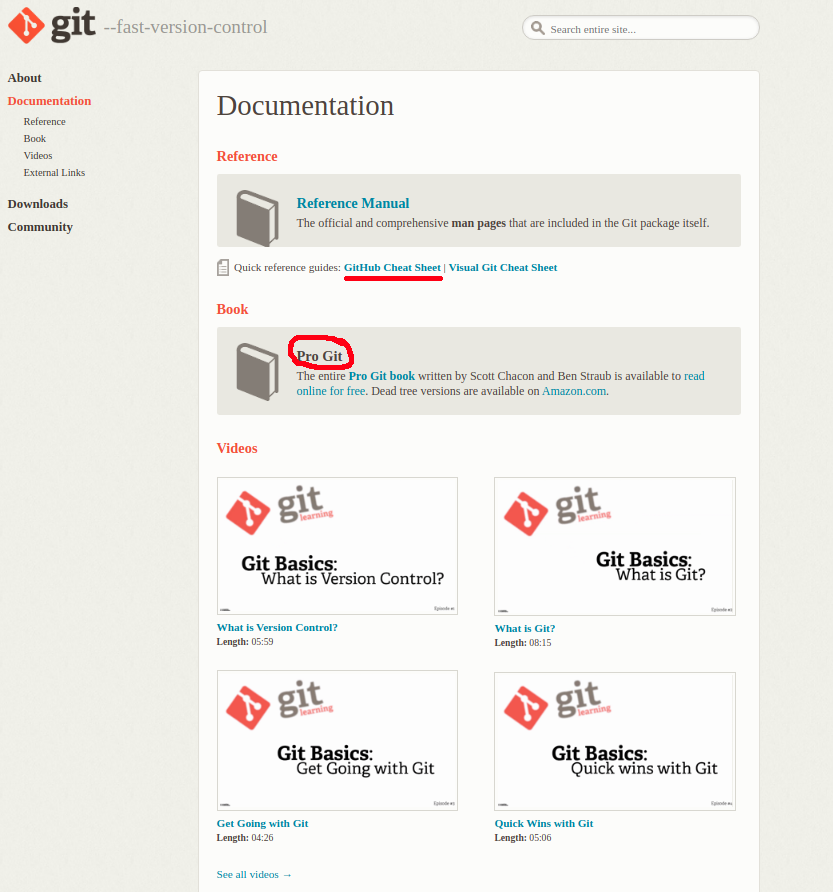
\includegraphics[scale=0.3]{images/git_ressources/doc.png}
\end{center}
\end{frame}

\begin{frame}
\frametitle{man giteveryday/gittutorial}
La commande "man giteveryday" vaut également le détour car elle est comme un petit "cheatsheet" intégré au terminal de commande.
\bigskip

La commande "man gittutorial" recense de nombreux tutoriels sur de nombreuses notions du versionnement par Git. Je recommande vivement d'explorer les suggestions de la section "SEE ALSO" en fin de page de ce manuel!
\end{frame}



%% --------------------- %%
%%        SECTION        %%
%% --------------------- %%
\AtBeginSection[]
{
  \begin{frame}
    \frametitle{Table of Contents}
    \tableofcontents[sectionstyle=show/hide,subsectionstyle=show/show/hide]
  \end{frame}
}
\section{Préparer son espace de travail}

% Subsection:
\subsection{Configurer Git}
\begin{frame}{Commande: git config $--$global user.name/user.email}
On ne peut pas faire de commit sans nom d'utilisateur et de mail! C'est une question de responsabilité.
\medskip

\underline{Syntaxe:} git config $--$global user.name "monNomUtilisateur"
\smallskip
\underline{Syntaxe:} git config $--$global user.email "monMail@Mailbox.com"
\medskip
\end{frame}

\begin{frame}{Commande: git config $--$global core.editor}
Par défaut Git ouvrira l'éditeur de texte Vim ou Nano lorsque vous écrirez les messages de vos commits (sauf si vous utilisez l'option -m, cf. \textit{git commit -m "..."}).\\
\medskip

Pour changer d'éditeur vous pouvez suivre les instructions de cette adresse : \url{https://git-scm.com/book/fr/v2/Commandes-Git-Installation-et-configuration}\\
\medskip

\underline{Exemple:} git config $--$global core.editor "'C:\textbackslash Program Files (x86)\textbackslash Windows NT\textbackslash Accessories\textbackslash wordpad.exe'"\\
\medskip

\textbf{IMPORTANT:} Remarquez dans cet exemple que les guillemets " entourent les simple quotes ' 
\end{frame}

\begin{frame}{Les alias de commandes}
\underline{Quelques alias recommandés:}
\begin{itemize} 
    \item[] git config $--$global alias.co checkout
    \item[] git config $--$global alias.br branch
    \item[] git config $--$global alias.ci commit
    \item[] git config $--$global alias.st status
\end{itemize}
\medskip
\underline{Un autre alias utile:}\\
git config $--$global alias.dog "log $--$all $--$decorate 
    											$--$oneline $--$graph"
\end{frame}

\begin{frame}{Lister et Supprimer des configurations}
\underline{Lister toutes ses clefs de configuration:}
\begin{itemize}
    \item[] git config $--$list
\end{itemize}
\medskip
\underline{Supprimer une configuration associée à une clef:}
\begin{itemize}
    \item[] git config $--$global $--$unset <clef>
    \footnote[frame]{Exemples:
    	\begin{itemize}
    	\item[] \textit{git config $--$global $--$unset core.editor}
    	\item[] \textit{git config $--$global $--$unset alias.st}
		\end{itemize}}
\end{itemize}
\medskip
\underline{Lister toutes les clefs de configuration possibles de Git:}
\begin{itemize}
    \item[] git help $--$config
\end{itemize}

\end{frame}

% Subsection:
\subsection{Initialiser le suivi des modifications ou cloner un projet}
\begin{frame}[fragile]{Commande: git init}
La commande "git init" crée le dossier caché .git/ contenant tous les fichiers dont Git a besoin pour offrir ses services:

    \begin{mdframed}[style=Bash]
    \begin{lstlisting}[style=Bash, caption={Contenu du dossier .git/}]
crex@crex:~/projects/test$ git init
Initialized empty Git repository in /home/crex/projects/test/.git/

crex@crex:~/projects/test/.git$ ls
branches  config  description  HEAD  hooks  info  objects  refs
    \end{lstlisting}
    \end{mdframed}
\end{frame}



%% --------------------- %%
%%        SECTION        %%
%% --------------------- %%
\AtBeginSection[]
{
  \begin{frame}
    \frametitle{Table of Contents}
    \tableofcontents[sectionstyle=show/hide,subsectionstyle=show/show/hide]
  \end{frame}
}
\section{La boucle de travail local}

% Subsection:
\subsection{Gérer le suivi des modifications}
\begin{frame}
\frametitle{Les trois (+1) états du suivi des modifications}

\begin{center}
    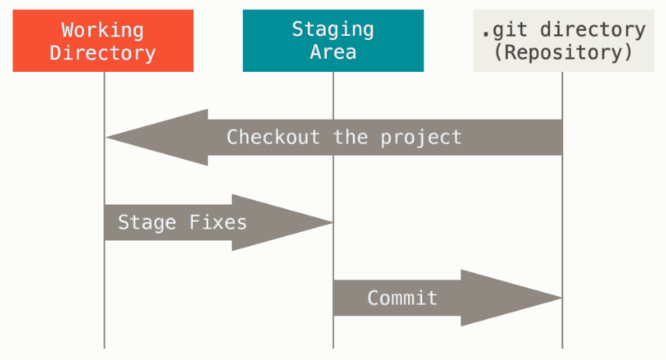
\includegraphics[scale=0.4]{images/boucle_locale/threeStates.png}
\end{center}

\end{frame}

\begin{frame}
\frametitle{Commande: git status}
La commande "git status" permet de savoir dans quel état se situent tous les fichiers du projet depuis la racine du projet. On remarque plusieurs choses:

\begin{itemize}
    \item Le suivi des modifications concerne par défaut tous les fichiers du projet en partant du dossier où se trouve le dossier .git/
    \item Par défaut aucun fichier n'est suivi, il faut préciser à Git les fichiers dont on souhaite suivre les modifications
    \item Si un fichier n'a pas été modifié et qu'il est suivi, il n'apparaît pas dans l'affichage de "git status"
    \item Un fichier non suivi continuera d'apparaître à chaque affichage de "git status"
\end{itemize}

\end{frame}

\begin{frame}[fragile]
\frametitle{Commande: git status}

    \begin{mdframed}[style=Bash]
    \begin{lstlisting}[style=Bash, caption={Tout premier appel à git status}]
crex@crex:~/projects/test$ git st
On branch master

No commits yet

Untracked files: (use "git add <file>..." to include in what will be committed)
	test.txt
	test2.txt

nothing added to commit but untracked files present (use "git add" to track)
    \end{lstlisting}
    \end{mdframed}

\end{frame}


\begin{frame}[fragile]
\frametitle{Commande: git status}

    \begin{mdframed}[style=Bash]
    \begin{lstlisting}[style=Bash, caption={git status après ajout au suivi de test.txt}]
crex@crex:~/projects/test$ git st
On branch master
No commits yet

Changes to be committed: (use "git rm --cached <file>..." to unstage)
	new file:   test.txt

Untracked files: (use "git add <file>..." to include in what will be committed)
	test2.txt
    \end{lstlisting}
    \end{mdframed}

\end{frame}


\begin{frame}[fragile]
\frametitle{Commande: git status}

    \begin{mdframed}[style=Bash]
    \begin{lstlisting}[style=Bash, caption={git status après commit}]
crex@crex:~/projects/test$ git st
On branch master
Untracked files:
  (use "git add <file>..." to include in what will be committed)
	test2.txt
nothing added to commit but untracked files present (use "git add" to track)
    \end{lstlisting}
    \end{mdframed}

\end{frame}


\begin{frame}[fragile]
\frametitle{Commande: git status}

    \begin{mdframed}[style=Bash]
    \begin{lstlisting}[style=Bash, caption={git status modification de test.txt}]
crex@crex:~/projects/test$ git st
On branch master
Changes not staged for commit: (use "git add <file>..." to update what will be committed) (use "git restore <file>..." to discard changes in working directory)
   modified:   test.txt

Untracked files: (use "git add <file>..." to include in what will be committed)
	test2.txt
    \end{lstlisting}
    \end{mdframed}

\end{frame}

\begin{frame}[fragile]
\frametitle{Le fichier .gitignore}
Le fichier .gitignore permet d'ignorer des fichiers du suivi des modifications. Les "wildcards" y sont autorisées:
\medskip
\begin{mdframed}[style=Bash]
    \begin{lstlisting}[style=Bash, caption={Contenu du dossier .git/}]
crex@crex:~/projects/avlTreesL3Project$ cat .gitignore 
*#*
*~

# Pour l'exemple:
*.cmi
!toto.cmi
    \end{lstlisting}
    \end{mdframed}
\end{frame}

\begin{frame}
\frametitle{Ajouter/Retirer du staging ou du suivi}

\underline{Pour ajouter au staging:}
\smallskip
\begin{itemize}
    \item[] git add <nom\_fichier>
    \item[] git add -A
\end{itemize}
\bigskip

\underline{Pour retirer du staging:}
\smallskip
\begin{itemize}
    \item[] git reset $--$ <nom\_fichier>
    \item[] git reset
\end{itemize}
\bigskip

\underline{Pour retirer un fichier du suivi des modifications:}
\smallskip
\begin{itemize}
    \item[] git rm $--$cached <nom\_fichier>
\end{itemize}
\end{frame}

% Subsection:
\subsection{Enregistrer une version}

\begin{frame}{Commande: git commit}
La commande git commit permet de sauvegarder l'ensemble des fichiers suivis en une version nommée automatiquement et ajoutée à l'historique des versions:
\smallskip
\begin{itemize}
    \item On doit toujours indiquer un message lors d'un commit\\
    \item Ce message doit expliquer ce qui a été fait
    \item Ce message sera visible de tous ceux qui auront votre projet (y compris sur le dépôt distant)
    \item Un "commit" est donc un engagement, vous engagez votre responsabilité
\end{itemize}
\end{frame}

\begin{frame}{Commande: git commit}
La commande \textit{git commit} admet plusieurs options et syntaxes:
\begin{itemize}
	\item git commit => ouvre l'éditeur de texte indiqué dans la clé de configuration 	          \textit{core.editor} pour vous permettre d'écrire votre message et enregistre 
	      ce qui était dans le staging area
	\item git commit -m "..." => enregistre ce qui était dans le staging area avec le 
	      message passé en paramètre
	\item git commit -a => combinaison\footnote[frame]{Exception faite que les fichiers non suivis ne seront pas commités ici!} \textit{git add -A} et \textit{git commit}
	\item git commit -am "..." => combinaison \textit{git add -A} et \textit{git commit -m "..."}
\end{itemize}
\end{frame}


\begin{frame}{Commande git commit $--$amend}
Du fait de l'importance de ces commits et des messages qui y sont associés, Git fournit un moyen de corriger le dernier commit grâce à l'option \textit{$--$amend}:
\begin{center}
	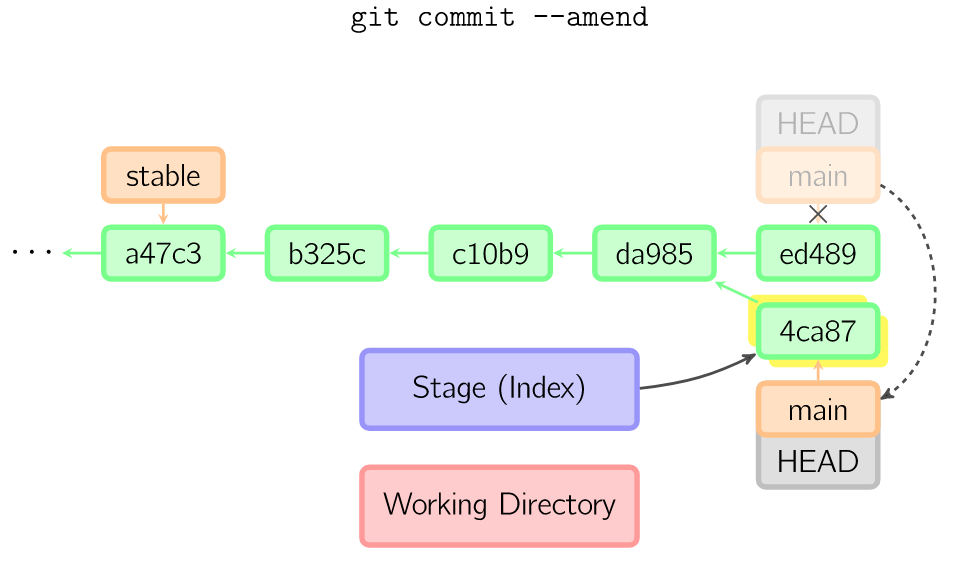
\includegraphics[scale=0.2]{gitCommitAmend.png}
\end{center}
\underline{NB:} Il n'est possible de corriger que le dernier commit.\\
\underline{NB2:} Par corriger on sous-entend "corriger le message" ou bien "ajouter d'autres changements au dernier commit".
\end{frame} 




%% --------------------- %%
%%        SECTION        %%
%% --------------------- %%
\AtBeginSection[]
{
  \begin{frame}
    \frametitle{Table of Contents}
    \tableofcontents[sectionstyle=show/hide,subsectionstyle=show/show/hide]
  \end{frame}
}
\section{Consulter des changements ou des versions}

% Subsection:
\subsection{Savoir qui a fait quoi sur un fichier}

\begin{frame}[fragile]{Commande: git blame <nom\_fichier>}
La commande \textit{git blame} suivi du nom d'un fichier permet d'afficher, ligne par ligne, qui a fait quoi (et quand) sur un fichier donné. Exemple:
\begin{mdframed}[style=Bash]
\begin{lstlisting}[style=Bash, caption={Exemple de git blame}]
e53bccf9 codes/..  (Florian 2021-04-11) public function construct()
f9f89eca codes/..  (Florian 2021-04-03) {
f9f89eca codes/..  (Florian 2021-04-03)  $em = $entityMan;
f9f89eca codes/..  (Florian 2021-04-03)  $user = getUser();
dc1bdd2a codes/..  (Florian 2021-04-08)  $globalUser->check($user);
f9f89eca codes/..  (Florian 2021-04-03) }
5e648da3 codes/..  (Florian 2021-03-31) 
eb8986af codes/..  (frafraA 2021-04-03) /**
268e35ac codes/..  (frafraA 2021-04-03)  * @Route("/manageAccount")
eb8986af codes/..  (frafraA 2021-04-03)  */
268e35ac codes/..  (frafraA 2021-04-03)  public function f(): Resp
\end{lstlisting}
\end{mdframed}
\end{frame}

% Subsection:
\subsection{L'historique des versions}
\begin{frame}[fragile]
\frametitle{Commande: git log}

La commande \textit{git log} permet d'afficher l'historique des versions. Ci-dessous un extrait d'un historique de version.
\begin{mdframed}[style=Bash]
    \begin{lstlisting}[style=Bash, caption={Exemple de bon message de commit}]
commit a3961497bd9c7ca94212922a46729a9410568eb8
Merge: 708c2e418142 fe0af09074bf
Author: Linus Torvalds <torvalds@linux-foundation.org>
Date:   Wed Feb 10 11:58:21 2021 -0800
    Merge tag 'acpi-5.11-rc8' of git://git.kernel.org/pub/scm/linux/kernel/git/rafael/linux-pm
    Pull ACPI fix from Rafael Wysocki:
     "Revert a problematic ACPICA commit that changed the code to attempt to update memory regions which may be read-only on some systems (Ard Biesheuvel)" [...]
    \end{lstlisting}
\end{mdframed}
\end{frame}

% Subsection:
\subsection{Les différences entre versions}
\begin{frame}{Commande: git diff}

\textit{git diff} montre ce qui a été ajouté/supprimé en partant du <nom\_commit1> jusqu'au <nom\_commit2>. \textit{git diff} sans aucun paramètre montre la différence en partant de la version dans le "staging area" et les fichiers actuels du dossier, etc. : 
\begin{center}
	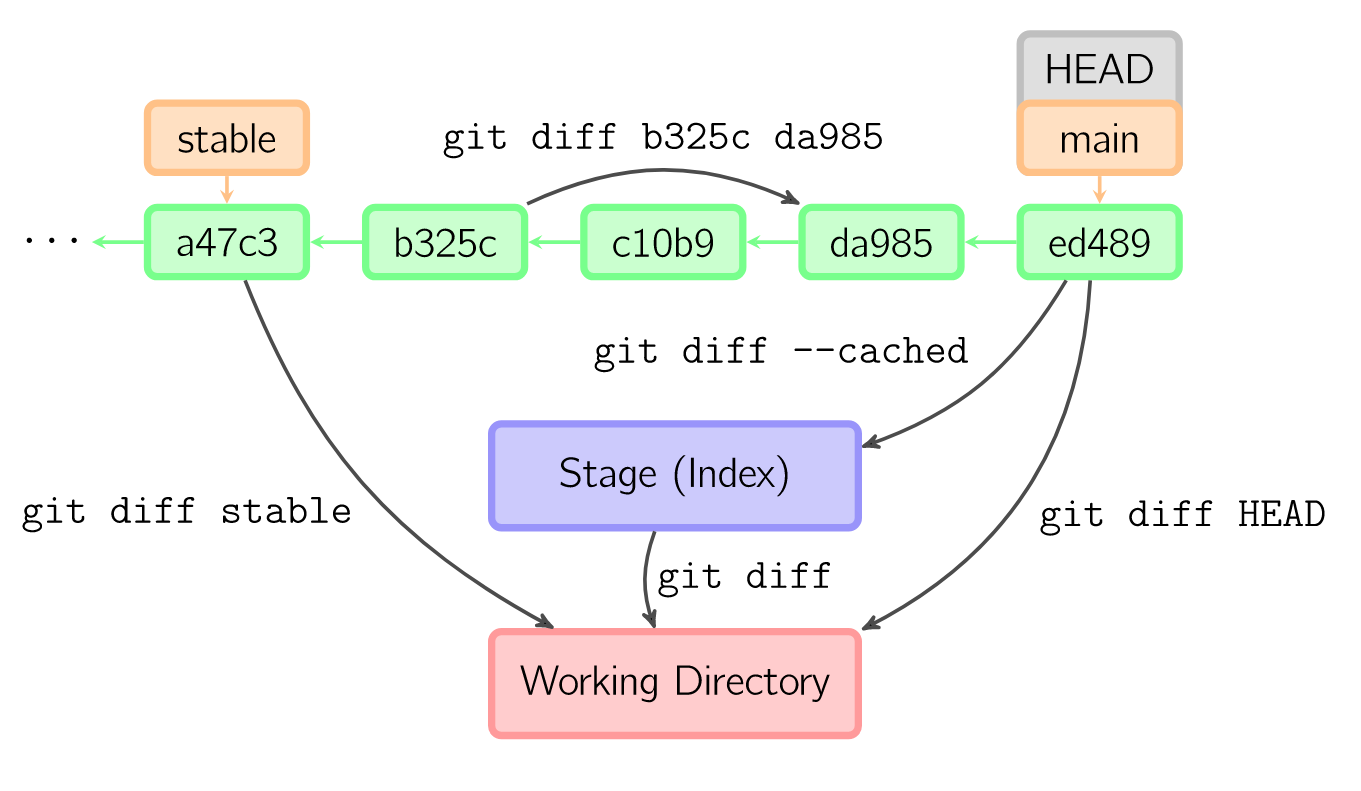
\includegraphics[scale=0.15]{gitDiff.png}
\end{center}
\end{frame}


% Subsection:
\subsection{Naviguer entre des versions}
\begin{frame}{Commande: git checkout <nom\_commit>}

La commande "git checkout <nom\_commit>" permet de déplacer le pointeur "HEAD". Lorsque le pointeur "HEAD" est déplacé cela met à jour les fichiers pour correspondre la version pointée:
\begin{center}
    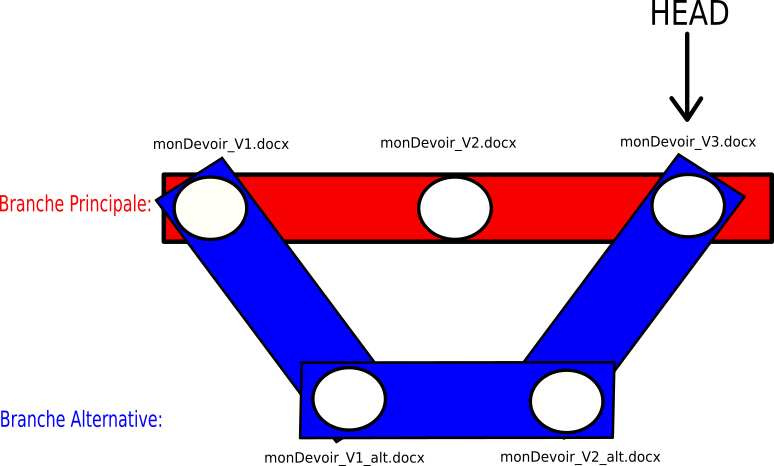
\includegraphics[scale=0.45]{images/consulter_versions/secondScenario_branches.png}
\end{center}
\end{frame}

\begin{frame}{À propos des noms de commit}
Il y a plusieurs façons d'obtenir un nom de commit:
\begin{itemize}
    \item Le nom absolu: "git log" + vous prenez les 4 ou 5 premiers caractères (inutile de donner toute la clef!)
    \item Le nom relatif: Exemple HEAD$\sim$2\string^3 => il vaut pour un numéro de commit! Seule différence: il est relatif
\end{itemize}
\end{frame}

\begin{frame}{Illustration des noms de commits relatifs}
    \begin{center}
        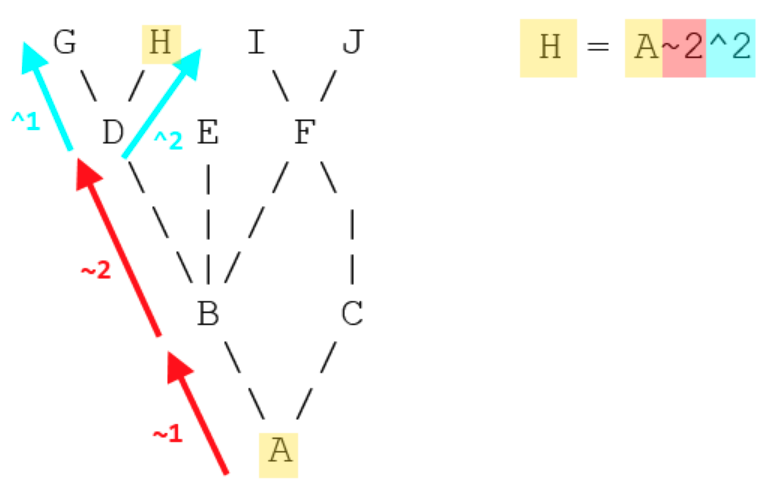
\includegraphics[scale=0.35]{images/nomCommits/nomCommitRelatif.png}
    \end{center}
\end{frame}

\begin{frame}{Que signifie "la tête est détachée"?}
    \begin{center}
        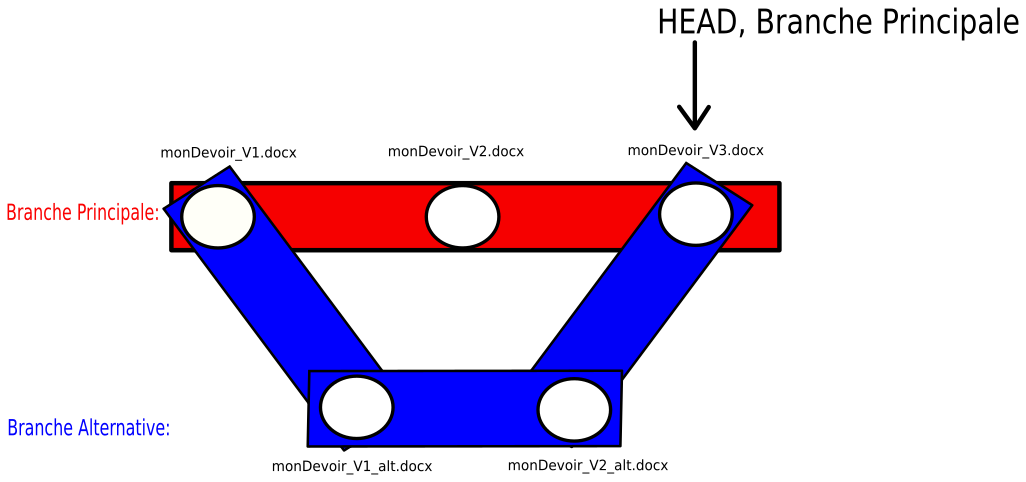
\includegraphics[scale=0.35]{images/detachedHead/detachedHead0.png}
    \end{center}
\end{frame}

\begin{frame}{Que signifie "la tête est détachée"?}
    \begin{center}
        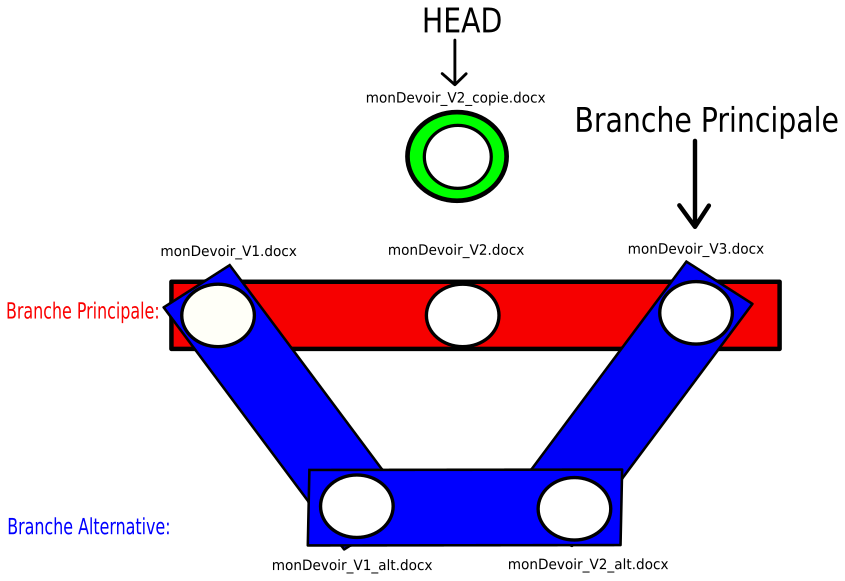
\includegraphics[scale=0.35]{images/detachedHead/detachedHead1.png}
    \end{center}
\end{frame}


\begin{frame}[fragile]{Qu'ai-je le droit de faire avec une tête détachée?}

\begin{mdframed}[style=Bash]
\begin{lstlisting}[style=Bash, caption={Des droits spéciaux avec une tête détachée}]
crex@crex:~/projects/matlab(main)$ git checkout a1a8a9
A	test
Note: switching to 'a1a8a9'.

You are in 'detached HEAD' state. You can look around, make 
experimental changes and commit them, and you can discard 
any commits you make in this state without impacting any branches 
by switching back to a branch.

If you want to create a new branch to retain commits you create, 
you may do so (now or later) by using -c with the switch command. 
Example:
  git switch -c <new-branch-name>
Or undo this operation with:
  git switch -

Turn off this advice by setting config variable advice.detachedHead to false
HEAD is now at a1a8a9d Initial commit
\end{lstlisting}
\end{mdframed}
\end{frame}

\begin{frame}{Qu'ai-je le droit de faire avec une tête détachée?}
    \begin{center}
        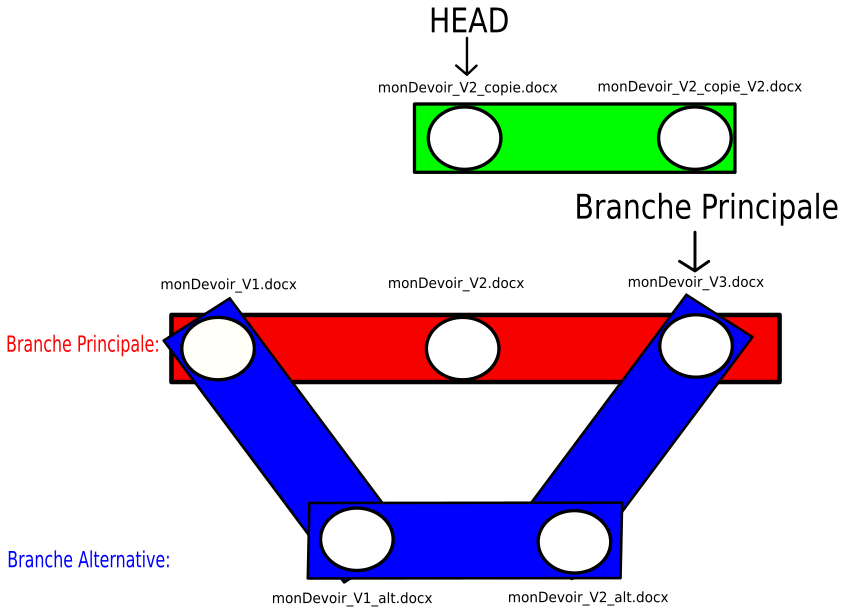
\includegraphics[scale=0.35]{images/detachedHead/detachedHead2.png}
    \end{center}
\end{frame}

\begin{frame}{Qu'ai-je le droit de faire avec une tête détachée?}
    \begin{center}
        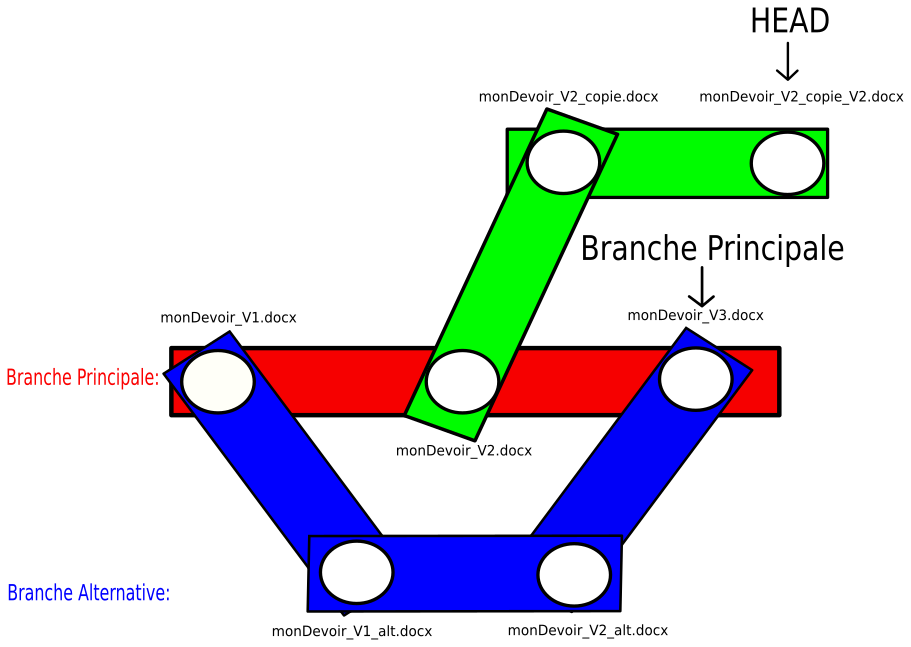
\includegraphics[scale=0.35]{images/detachedHead/detachedHead3.png}
    \end{center}
\end{frame}



%% --------------------- %%
%%        SECTION        %%
%% --------------------- %%
\AtBeginSection[]
{
  \begin{frame}
    \frametitle{Table of Contents}
    \tableofcontents[sectionstyle=show/hide,subsectionstyle=show/show/hide]
  \end{frame}
}
\section{Annuler des versions}


% Subsection:
\subsection{Annulez au lieu de supprimer!}
\begin{frame}{Commande: git revert -n <older\_id>\string^..HEAD}
Cette commande crée un commit qui contient l'annulation de tous les changements des commits spécifiés dans l'intervalle \textit{<older\_id>\string^..HEAD}\\
\medskip 
C'est-à-dire l'intervalle: ]<parent\_of\_older\_id>; HEAD]\\ \hspace{3.9cm}(ie. [<older\_id>; HEAD])\\ 
\medskip
Retirez le "\string^" pour obtenir l'intervalle ]<older\_id>; HEAD]
\vspace{0.4cm}


\textbf{IMPORTANT:} L'option "-n" évite la création automatique d'un commit. Cela présente plusieurs avantages:
\begin{enumerate}
	\item Ça laisse le temps de réfléchir à son annulation
	\item Ça évite une "cascade" de commits d'annulations
	\item Si vous voulez "annuler l'annulation" vous pouvez le faire très rapidement
	      avec la commande \textit{git revert HEAD}
\end{enumerate}
\end{frame}


% Subsection:
\subsection{Annuler un changement apporté par une version donnée}
\begin{frame}{Annuler un changement apporté par une version donnée}
	Cette question ne sera pas abordée ici car elle demande une assez bonne connaissance de Git et notamment de la résolution des conflits. Elle est abordée dans le module "bonus" associé à ce module. 
\end{frame}



%% --------------------- %%
%%        SECTION        %%
%% --------------------- %%
\AtBeginSection[]
{
  \begin{frame}
    \frametitle{Table of Contents}
    \tableofcontents[sectionstyle=show/hide,subsectionstyle=show/show/hide]
  \end{frame}
}
\section{Supprimer des changements ou des versions}

% Subsection:
\subsection{Supprimer des changements sur un seul fichier}
\begin{frame}{git restore <file>}
Permet de restaurer un seul fichier à l'état de son dernier commit.\\
\medskip

\underline{Cas concret:} Vous travaillez sur votre code, vous sauvegardez et la fin de la journée arrive. Vous ne voulez pas "commiter" vos changements car vous n'avez pas encore eu le temps de tester vos ajouts...\\
\medskip

Le lendemain matin vous reprenez votre code et il est truffé de bug. Vous voulez "revert" uniquement ce fichier (les autres ont l'air bon) => \textit{git restore <nom\_fichier>}
\end{frame}


% Subsection:
\subsection{Supprimer des changements sur tous les fichiers}
\begin{frame}{Commande: git reset $--$hard (sans paramètre)}
La commande \textit{git reset $--$hard} sans paramètre permet d'annuler tous les changements en cours dans votre dossier de travail. L'historique des modifications n'est pas touché!\\
\medskip

C'est une façon très pratique de repartir de 0 quand on n'est pas satisfait de ce qu'on a écrit...
\end{frame}


% Subsection:
\subsection{Supprimer des versions}
\begin{frame}{Commande: git reset $--$hard <numero\_commit>}
La commande \textit{git reset $--$hard <numero\_commit>} permet d'annuler tous les commits qui ont été faits après le commit spécifié et de faire revenir ses fichiers à l'état du commit spécifié.
\medskip

Il n'est pas utile d'indiquer l'entièreté du numéro du commit, seuls les 4 (ou 5) premiers caractères suffisent.
\medskip

\textbf{ATTENTION!} C'est une commande très dangereuse... Ce qui est perdu est perdu définitivement! À n'utiliser qu'en cas de dernier recours.
\end{frame}



\end{document}